%!TEX root = ../../report.tex
\chapter{Integration into MIR100 software}
%\begin{figure}
%	\centering
%	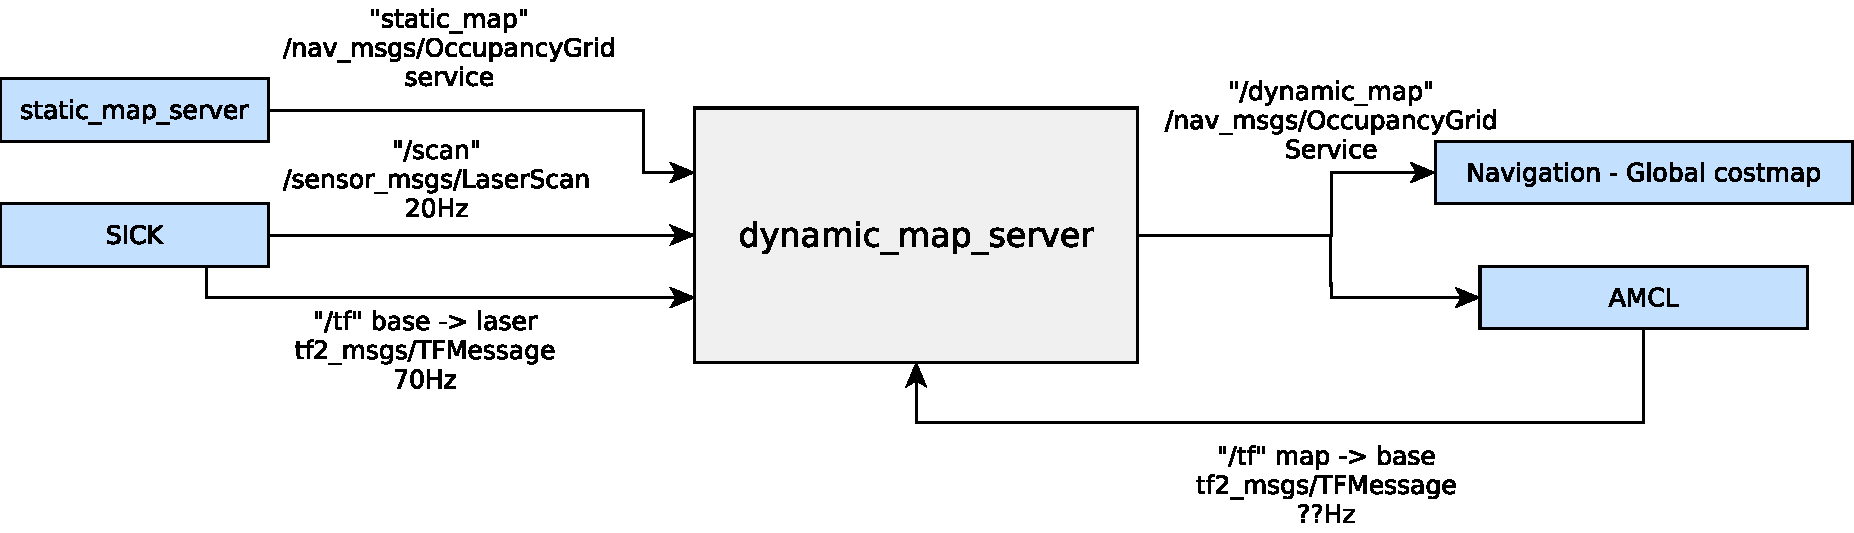
\includegraphics[width=0.6\linewidth]{figures/dynamic_map_mir_interface}
%	\caption{Crossing point determined using P4P and an offset from the QR tag in its frame.}
%	\label{fig:dyn_map}
%\end{figure}

\section{Layered Costmap}
To ease the integration the update from static to dynamic map should involve as few changes to the original system as possible. 
Since different sensor source have different pros and cons it should be possible to extend the solution in the future easily with more sensors. 


